\documentclass[12pt,a4paper]{report}

% ===================== PACKAGES =====================
\usepackage[a4paper,margin=1in]{geometry}
\usepackage{times}
\usepackage[T1]{fontenc}
\usepackage[utf8]{inputenc}
\usepackage{graphicx}
\usepackage{amsmath,amssymb}
\usepackage{booktabs}
\usepackage{array}
\usepackage{longtable}
\usepackage{xcolor}
\usepackage{fancyhdr}
\usepackage{titlesec}
\usepackage{tocloft}
\usepackage{enumitem}
\usepackage{listings}
\usepackage{caption}
\usepackage{subcaption}
\usepackage{hyperref}
\usepackage{tikz}
\usetikzlibrary{positioning,arrows.meta,shapes.geometric,fit,backgrounds}
\usepackage{float}
\usepackage{setspace}
\usepackage{multirow}
\usepackage{colortbl}
\usepackage{pifont}
\usepackage{pgfplots}
\pgfplotsset{compat=1.17}

% ===================== COLORS =====================
\definecolor{navy}{RGB}{20,40,90}
\definecolor{steel}{RGB}{70,110,160}
\definecolor{lightgray}{RGB}{245,245,245}
\definecolor{codebg}{RGB}{247,247,250}
\definecolor{codekw}{RGB}{0,70,140}
\definecolor{codecom}{RGB}{110,110,110}
\definecolor{codestr}{RGB}{160,40,40}

% ===================== HEADER/FOOTER =====================
\setlength{\headheight}{14pt}
\pagestyle{fancy}
\fancyhf{}
\renewcommand{\headrulewidth}{0.4pt}
\fancyhead[L]{\small\itshape CNN Image Classification on FashionMNIST}
\fancyhead[R]{\small\itshape Student ID: 220141}
\fancyfoot[C]{\thepage}

% ===================== SECTION STYLING =====================
\titleformat{\chapter}[display]
  {\normalfont\bfseries\color{navy}}
  {\Large\chaptertitlename\ \thechapter}
  {10pt}{\Huge}
\titleformat{\section}
  {\normalfont\Large\bfseries\color{navy}}{\thesection}{1em}{}
\titleformat{\subsection}
  {\normalfont\large\bfseries\color{steel}}{\thesubsection}{1em}{}

% ===================== CODE LISTING STYLE =====================
\lstdefinestyle{python}{
  language=Python,
  backgroundcolor=\color{codebg},
  basicstyle=\ttfamily\footnotesize,
  keywordstyle=\color{codekw}\bfseries,
  commentstyle=\color{codecom}\itshape,
  stringstyle=\color{codestr},
  numbers=left,
  numberstyle=\tiny\color{gray},
  numbersep=8pt,
  frame=single,
  rulecolor=\color{gray!40},
  breaklines=true,
  breakatwhitespace=false,
  showstringspaces=false,
  tabsize=4,
  captionpos=b,
  xleftmargin=1.5em,
  framexleftmargin=1.5em
}
\lstset{style=python}

% ===================== TITLE INFO =====================
\title{
  \vspace{-2cm}
  {\color{navy}\rule{\linewidth}{2pt}}\\[0.4cm]
  {\Huge\bfseries Convolutional Neural Network--Based\\ Image Classification on the FashionMNIST\\ Dataset with Real-World Generalization\\ Analysis}\\[0.4cm]
  {\color{navy}\rule{\linewidth}{2pt}}\\[1cm]
  {\large A Comprehensive Technical Report on Model Design,\\ Training, Evaluation, and Domain-Shift Analysis}
}
\author{Student ID: 220141}
\date{\today}

\begin{document}

% ===================== TITLE PAGE =====================
\begin{titlepage}
\centering
\vspace*{1cm}
{\color{navy}\rule{\linewidth}{3pt}}\\[0.6cm]
{\Huge\bfseries Convolutional Neural Network--Based Image Classification on the FashionMNIST Dataset}\\[0.6cm]
{\Large\itshape with Real-World Generalization and Error Analysis}\\[0.6cm]
{\color{navy}\rule{\linewidth}{3pt}}\\[2cm]


\begin{tikzpicture}
\node[draw=navy, thick, rounded corners, inner sep=14pt, fill=lightgray] {
  \begin{minipage}{0.7\linewidth}
  \centering
  \textbf{\large Deep Learning \& Computer Vision Coursework Report}\\[0.3cm]
  \textit{Custom CNN Architecture Design, Training Diagnostics,\\ Confusion Matrix Analysis, and Out-of-Distribution\\ Evaluation on Phone-Captured Photographs}
  \end{minipage}
};
\end{tikzpicture}

\vspace{2.5cm}

{\Large\bfseries Submitted by}\\[0.3cm]
{\Large Student ID: 220141}\\[1.5cm]

{\Large\bfseries Project Repository}\\[0.3cm]
{\large\ttfamily github.com/just-abir/220141\_CNN\_Image\_Classification}\\[1.5cm]

{\Large\bfseries Framework}\\[0.3cm]
{\large PyTorch / Torchvision}\\[2cm]

\vfill
{\large \today}\\[0.3cm]
{\color{navy}\rule{0.6\linewidth}{1.5pt}}
\end{titlepage}

% ===================== FRONT MATTER =====================
\pagenumbering{roman}

\chapter*{Declaration}
\addcontentsline{toc}{chapter}{Declaration}
I hereby declare that the work presented in this report, titled \emph{``Convolutional Neural Network--Based Image Classification on the FashionMNIST Dataset with Real-World Generalization Analysis,''} is the result of my own investigation, except where otherwise stated. All source code, experiments, figures, and analyses were carried out by me as part of a deep learning and computer vision coursework assignment. The FashionMNIST dataset used is a publicly available benchmark dataset released by Zalando Research, and any third-party resources referenced are cited accordingly. The custom phone-photograph dataset used for out-of-distribution evaluation was personally captured, labeled, and hosted in the linked public repository.

\vspace{1cm}
\noindent Signed: \underline{\hspace{5cm}} \\[0.3cm]
\noindent Student ID: 220141 \\[0.3cm]
\noindent Date: \today

\chapter*{Abstract}
\addcontentsline{toc}{chapter}{Abstract}
This report presents the complete design, implementation, training, and evaluation of a convolutional neural network (CNN) for multi-class image classification on the FashionMNIST dataset. The proposed architecture consists of two convolutional layers, each followed by ReLU activation and max-pooling, feeding into a fully connected classification head regularized with dropout. The network was trained for a total of twenty epochs across two consecutive training phases using the Adam optimizer with a learning rate of $0.001$ and cross-entropy loss. The model achieved a peak validation accuracy of approximately $92.43\%$ and a final training accuracy of $97.97\%$, revealing a clear overfitting trend beyond epoch ten. A confusion matrix was constructed on the full $10{,}000$-image standard test set to quantify per-class performance, exposing systematic confusion among visually similar upper-body garment classes. Beyond the standard benchmark evaluation, this report undertakes a novel out-of-distribution robustness study: ten real-world phone-camera photographs of clothing items were manually labeled and passed through the trained network, after diagnosing and correcting a critical background-inversion preprocessing bug. Despite strong benchmark performance, the model achieved only $40\%$ accuracy on these real-world images, several of which were misclassified with extremely high confidence, illustrating a substantial domain gap between curated benchmark imagery and unconstrained real-world photography. This report documents the complete methodology, architecture rationale, training dynamics, quantitative and qualitative error analysis, and provides a critical discussion of the limitations of small-scale CNNs when deployed outside their training distribution, along with concrete recommendations for future improvement including data augmentation, batch normalization, early stopping, and background-aware preprocessing.

\vspace{0.5cm}
\noindent\textbf{Keywords:} Convolutional Neural Networks, FashionMNIST, Image Classification, PyTorch, Overfitting, Confusion Matrix, Domain Shift, Out-of-Distribution Generalization, Deep Learning.

\tableofcontents
\listoffigures
\listoftables

\chapter*{List of Abbreviations}
\addcontentsline{toc}{chapter}{List of Abbreviations}
\begin{tabular}{@{}ll@{}}
\textbf{CNN} & Convolutional Neural Network \\
\textbf{ReLU} & Rectified Linear Unit \\
\textbf{GPU} & Graphics Processing Unit \\
\textbf{CUDA} & Compute Unified Device Architecture \\
\textbf{Adam} & Adaptive Moment Estimation (optimizer) \\
\textbf{OOD} & Out-of-Distribution \\
\textbf{RGB} & Red-Green-Blue (color image format) \\
\textbf{FC} & Fully Connected (layer) \\
\textbf{SGD} & Stochastic Gradient Descent \\
\textbf{API} & Application Programming Interface \\
\end{tabular}

\clearpage
\pagenumbering{arabic}

% =====================================================
\chapter{Introduction}
% =====================================================

\section{Background and Motivation}
Image classification remains one of the foundational problems in computer vision, forming the backbone of countless downstream applications ranging from e-commerce product tagging to autonomous inspection systems. Convolutional Neural Networks (CNNs) have, since the introduction of architectures such as LeNet-5 and later AlexNet, become the de facto standard approach for extracting hierarchical spatial features directly from raw pixel data without the need for hand-engineered features.

The FashionMNIST dataset, introduced by Zalando Research as a drop-in replacement for the original MNIST handwritten digit dataset, provides a more challenging yet still compact benchmark: $28 \times 28$ grayscale images spanning ten categories of clothing and footwear. Its manageable size and class complexity make it an ideal sandbox for prototyping CNN architectures, studying training dynamics such as overfitting, and exploring evaluation methodologies such as confusion matrices and error analysis, all without the computational overhead of larger-scale datasets like ImageNet.

However, a benchmark dataset such as FashionMNIST — with its centered, background-free, uniformly-lit grayscale images — represents an idealized data distribution that rarely matches the conditions of real-world deployment. A central motivation of this project, therefore, is not only to build and train a competent CNN classifier on FashionMNIST itself, but to explicitly probe how well such a model generalizes when confronted with genuinely unconstrained input: photographs taken with an ordinary phone camera, under natural lighting, against non-uniform backgrounds, and without any of the careful curation applied to the benchmark dataset.

\section{Problem Statement}
Given a set of grayscale clothing images belonging to one of ten predefined categories, the objective is to design, train, and evaluate a convolutional neural network capable of accurately predicting the correct category label. In addition to standard benchmark evaluation, this project further investigates the following applied research question:

\begin{quote}
\itshape
``To what extent does a CNN trained exclusively on the clean, curated FashionMNIST benchmark generalize to real-world photographs of the same clothing categories, and what specific preprocessing and modeling factors influence this generalization gap?''
\end{quote}

\section{Objectives}
The specific objectives pursued in this project are as follows:

\begin{enumerate}[label=\arabic*.]
    \item Design a compact, trainable-from-scratch CNN architecture suitable for $28\times28$ grayscale image classification.
    \item Implement a complete PyTorch training pipeline, including data loading, augmentation-free preprocessing, loss computation, optimization, and per-epoch validation tracking.
    \item Train the network on the FashionMNIST training set and evaluate it on the corresponding held-out test set.
    \item Visualize training dynamics (loss and accuracy curves) to diagnose convergence behavior and potential overfitting.
    \item Construct and interpret a full $10\times10$ confusion matrix to characterize per-class prediction performance.
    \item Curate a small, independently labeled dataset of ten real-world phone photographs spanning all ten FashionMNIST categories.
    \item Diagnose and correct preprocessing incompatibilities (specifically, background/foreground color inversion) between the benchmark data distribution and real-world photographs.
    \item Quantitatively and qualitatively evaluate the trained model's performance on this out-of-distribution dataset, including per-image softmax confidence scores.
    \item Perform visual error analysis on both the standard test set and the custom photo set to identify systematic failure modes.
    \item Synthesize findings into actionable recommendations for improving real-world robustness of small CNN classifiers.
\end{enumerate}

\section{Scope of the Report}
This report is organized to walk through the project end-to-end: from dataset characteristics and preprocessing decisions, through architecture design and training configuration, to a detailed presentation and interpretation of results on both the standard benchmark and the custom out-of-distribution dataset. Particular emphasis is placed on the practical engineering challenges encountered — most notably the background-inversion bug affecting custom image preprocessing — and on a rigorous, evidence-based discussion of the resulting domain gap. The report closes with a critical discussion of limitations and a roadmap of concrete future improvements.

\section{Report Organization}
The remainder of this report is structured as follows. Chapter~2 reviews relevant background on CNNs and the FashionMNIST benchmark. Chapter~3 details the dataset and preprocessing pipeline. Chapter~4 presents the model architecture in full mathematical and implementation detail. Chapter~5 describes the training methodology and configuration. Chapter~6 presents quantitative results on the standard test set, including training curves and the confusion matrix. Chapter~7 presents the out-of-distribution evaluation on custom phone photographs. Chapter~8 performs a detailed qualitative error analysis. Chapter~9 discusses the findings in depth. Chapter~10 outlines limitations and future work. Chapter~11 concludes the report. Full source code is provided in the Appendix for reference and reproducibility.

% =====================================================
\chapter{Background and Literature Context}
% =====================================================

\section{Convolutional Neural Networks}
Convolutional Neural Networks are a class of deep learning models specifically designed to exploit the spatial structure of image data. Unlike fully connected networks, which treat each pixel as an independent input feature, CNNs apply learnable convolutional filters (kernels) that slide across the input image, producing feature maps that capture local spatial patterns such as edges, textures, and shapes. Stacking multiple convolutional layers allows the network to build increasingly abstract and semantically meaningful representations — early layers typically detect low-level features such as edges and corners, while deeper layers capture higher-level structures such as object parts and, eventually, whole-object representations.

Three components are central to nearly every CNN architecture:

\begin{itemize}
    \item \textbf{Convolutional layers}, which apply a set of learnable filters across the spatial dimensions of the input, producing feature maps via the discrete convolution (technically cross-correlation) operation.
    \item \textbf{Pooling layers} (commonly max-pooling), which downsample feature maps, reducing spatial dimensionality while retaining the most salient activations, thereby also providing a degree of translation invariance.
    \item \textbf{Fully connected layers}, typically placed at the end of the network, which combine the high-level spatial features into a final classification decision.
\end{itemize}

\section{The Role of Activation Functions}
Non-linear activation functions are essential for enabling CNNs to model complex, non-linear decision boundaries. The Rectified Linear Unit (ReLU), defined as

\begin{equation}
    \text{ReLU}(x) = \max(0, x)
\end{equation}

is used throughout the architecture presented in this report. ReLU is computationally inexpensive, mitigates the vanishing gradient problem relative to saturating activations such as sigmoid or tanh, and empirically accelerates convergence in deep networks.

\section{Regularization via Dropout}
Dropout \cite{srivastava2014dropout} is a regularization technique in which a randomly selected subset of neurons is deactivated (set to zero) during each training iteration, with probability $p$. This prevents co-adaptation of neurons and reduces overfitting by forcing the network to learn redundant, distributed representations rather than relying on any single neuron or narrow pathway. At inference time, dropout is disabled, and the layer instead scales the remaining activations to preserve the expected output magnitude. In this project, a dropout probability of $p = 0.25$ is applied to the first fully connected layer's output.

\section{Optimization with Adam}
The Adam optimizer \cite{kingma2014adam} combines the benefits of two other extensions of stochastic gradient descent: AdaGrad's per-parameter learning rate adaptation and RMSProp's use of a moving average of squared gradients. Adam maintains estimates of both the first moment (mean) and second moment (uncentered variance) of the gradients:

\begin{align}
    m_t &= \beta_1 m_{t-1} + (1-\beta_1) g_t \\
    v_t &= \beta_2 v_{t-1} + (1-\beta_2) g_t^2 \\
    \hat{m}_t &= \frac{m_t}{1-\beta_1^t}, \quad \hat{v}_t = \frac{v_t}{1-\beta_2^t} \\
    \theta_t &= \theta_{t-1} - \eta \frac{\hat{m}_t}{\sqrt{\hat{v}_t} + \epsilon}
\end{align}

where $g_t$ is the gradient at time step $t$, $\eta$ is the learning rate, and $\beta_1, \beta_2, \epsilon$ are hyperparameters (commonly $0.9$, $0.999$, and $10^{-8}$ respectively). Adam's adaptive per-parameter step sizes make it a robust default choice for training CNNs without extensive learning-rate tuning, which motivated its selection for this project.

\section{Cross-Entropy Loss for Multi-Class Classification}
For a $K$-class classification problem, the categorical cross-entropy loss between the predicted class probability distribution $\hat{y}$ (obtained via softmax over the logits) and the true one-hot label $y$ is defined as:

\begin{equation}
    \mathcal{L}_{\text{CE}} = -\sum_{k=1}^{K} y_k \log(\hat{y}_k)
\end{equation}

In PyTorch, \texttt{nn.CrossEntropyLoss} conveniently combines the softmax computation and the negative log-likelihood loss into a single numerically stable operation, operating directly on raw logits rather than requiring an explicit softmax layer within the model.

\section{The FashionMNIST Benchmark}
FashionMNIST was released as a more challenging, real-world-relevant alternative to the original MNIST handwritten digits dataset, which had become widely regarded as \emph{``too easy''} for modern architectures, with even simple classifiers achieving near-perfect accuracy. FashionMNIST retains MNIST's exact image format ($28\times28$ grayscale, 60,000 training images, 10,000 test images) while replacing digit classes with ten categories of clothing and accessories, thereby preserving drop-in compatibility with existing MNIST-based pipelines while substantially raising the classification difficulty.

\section{Domain Shift and Out-of-Distribution Generalization}
A recurring theme in applied machine learning is the gap between performance on a held-out test set drawn from the same distribution as the training data, and performance on data drawn from a different — but related — distribution, commonly referred to as \emph{domain shift} or \emph{distribution shift}. Models that perform strongly on in-distribution benchmarks frequently suffer significant performance degradation when exposed to inputs that differ in acquisition conditions, such as lighting, background, sensor characteristics, or framing. This project's custom phone-photograph evaluation is explicitly designed to surface and quantify this phenomenon in a controlled, small-scale setting.

% =====================================================
\chapter{Dataset and Preprocessing}
% =====================================================

\section{FashionMNIST Dataset Description}
The FashionMNIST dataset is accessed directly through \texttt{torchvision.datasets.FashionMNIST}, which automatically downloads and caches the dataset locally. It consists of:

\begin{itemize}
    \item \textbf{60,000} training images.
    \item \textbf{10,000} test images.
    \item Each image is $28 \times 28$ pixels, single-channel grayscale, pixel values originally in $[0, 255]$.
    \item \textbf{10} mutually exclusive classes, as summarized in Table~\ref{tab:classes}.
\end{itemize}

\begin{table}[H]
\centering
\caption{FashionMNIST class labels}
\label{tab:classes}
\begin{tabular}{@{}cl@{}}
\toprule
\textbf{Label Index} & \textbf{Class Name} \\
\midrule
0 & T-shirt/top \\
1 & Trouser \\
2 & Pullover \\
3 & Dress \\
4 & Coat \\
5 & Sandal \\
6 & Shirt \\
7 & Sneaker \\
8 & Bag \\
9 & Ankle boot \\
\bottomrule
\end{tabular}
\end{table}

\section{Custom Phone-Photograph Dataset}
To evaluate real-world generalization, ten photographs of physical clothing and footwear items were captured using a smartphone camera and manually labeled according to the FashionMNIST class taxonomy. These images are hosted in the public GitHub repository \texttt{just-abir/220141\_CNN\_Image\_Classification} and are cloned programmatically at the start of the notebook execution. Table~\ref{tab:customset} lists the full custom dataset.

\begin{table}[H]
\centering
\caption{Custom phone-photograph dataset and ground-truth labels}
\label{tab:customset}
\begin{tabular}{@{}cll@{}}
\toprule
\textbf{\#} & \textbf{Filename} & \textbf{Ground-Truth Label} \\
\midrule
1  & \texttt{1\_Shoe.jpeg}        & Sneaker \\
2  & \texttt{02\_Shirt.jpg}       & Shirt \\
3  & \texttt{03\_Pant.jpg}        & Trouser \\
4  & \texttt{04\_Jacket.jpg}      & Coat \\
5  & \texttt{05\_sneaker.jpg}     & Sneaker \\
6  & \texttt{06\_pullover.jpg}    & Pullover \\
7  & \texttt{07\_Coat.png}        & Coat \\
8  & \texttt{08\_Pholo\_Shirt.jpg}& T-shirt/top \\
9  & \texttt{09\_dress.jpg}       & Dress \\
10 & \texttt{10\_Bag.jpeg}        & Bag \\
\bottomrule
\end{tabular}
\end{table}

\section{Standard Preprocessing Pipeline}
For FashionMNIST images, the following transformation pipeline is applied uniformly to both training and test sets:

\begin{lstlisting}[caption={Standard preprocessing transform}, label={lst:transform}]
transform = transforms.Compose([
    transforms.Grayscale(num_output_channels=1),
    transforms.Resize((28, 28)),
    transforms.ToTensor(),
    transforms.Normalize((0.5,), (0.5,))
])
\end{lstlisting}

Each stage of this pipeline serves a specific purpose:

\begin{enumerate}
    \item \textbf{Grayscale conversion} ensures single-channel input consistent with the network's first convolutional layer, which expects \texttt{in\_channels=1}.
    \item \textbf{Resizing} to $28\times28$ standardizes spatial dimensions to match FashionMNIST's native resolution.
    \item \textbf{Tensor conversion} rescales pixel intensities from $[0,255]$ integers to $[0,1]$ floating-point values and reshapes the array into PyTorch's channel-first tensor format.
    \item \textbf{Normalization} with mean $0.5$ and standard deviation $0.5$ maps pixel values into the range $[-1, 1]$, which is known empirically to improve gradient-based optimization stability.
\end{enumerate}

\section{The Custom Image Preprocessing Challenge}
\label{sec:invert}
A critical engineering challenge encountered during this project was a systematic misclassification of nearly all custom images when the standard transform (Listing~\ref{lst:transform}) was naively applied. Diagnostic visualization of the preprocessed tensors (Step 8.1--8.3 in the accompanying notebook) revealed the root cause: FashionMNIST images are rendered with a \textbf{black background and a light-colored garment silhouette}, whereas ordinary phone photographs typically exhibit the \textbf{opposite convention} — a light background (e.g., a table, wall, or floor) with a comparatively darker garment.

Left uncorrected, this color-convention mismatch causes the network to interpret the background, rather than the garment, as the dominant foreground signal — a catastrophic and silent failure mode, since the model still produces confident (but essentially meaningless) predictions.

\subsection{Auto-Invert Correction}
The corrected preprocessing function programmatically detects and corrects this mismatch by inspecting the mean pixel intensity of the resized, tensor-converted (but not yet normalized) image:

\begin{lstlisting}[caption={Auto-invert preprocessing for custom images}, label={lst:autoinvert}]
def load_custom_image(image_path, transform):
    image = Image.open(image_path).convert('L')   # grayscale
    image = transform(image)                        # resize + tensor

    # Auto-invert: if background is light, flip colors
    if image.mean() > 0.5:
        image = 1.0 - image

    # Normalize (same convention as training data)
    image = (image - 0.5) / 0.5

    image = image.unsqueeze(0)  # add batch dimension
    return image

custom_transform = transforms.Compose([
    transforms.Resize((28, 28)),
    transforms.ToTensor()
])
\end{lstlisting}

This heuristic assumes that a mean pixel intensity greater than $0.5$ (on the $[0,1]$ scale, prior to normalization) indicates a predominantly light background, in which case the image is inverted via $1 - x$ before normalization. While simple, this heuristic proved sufficient to bring the custom images into visual alignment with the FashionMNIST convention, as confirmed by direct visualization of the preprocessed tensors (see Chapter~7).

\section{Data Loading Configuration}
Both the training and test FashionMNIST sets are wrapped in PyTorch \texttt{DataLoader} objects with the configuration shown in Table~\ref{tab:loader}.

\begin{table}[H]
\centering
\caption{DataLoader configuration}
\label{tab:loader}
\begin{tabular}{@{}lcc@{}}
\toprule
\textbf{Loader} & \textbf{Batch Size} & \textbf{Shuffle} \\
\midrule
Training loader & 64 & True \\
Test loader     & 64 & False \\
\bottomrule
\end{tabular}
\end{table}

Shuffling is enabled for the training loader to ensure each mini-batch is a randomized sample of the training distribution, preventing the model from learning spurious ordering-dependent patterns. The test loader is left unshuffled since evaluation order does not affect correctness and a fixed order simplifies result inspection (e.g., for the confusion matrix and error analysis).

% =====================================================
\chapter{Model Architecture}
% =====================================================

\section{Design Philosophy}
The architecture adopted in this project follows a deliberately compact design philosophy appropriate for the low-resolution, single-channel nature of FashionMNIST images. Rather than adapting a large, ImageNet-scale backbone, a purpose-built two-convolutional-block CNN was implemented, prioritizing:

\begin{itemize}
    \item \textbf{Parameter efficiency}, keeping the model small enough to train from scratch in a handful of epochs on modest hardware.
    \item \textbf{Sufficient representational capacity} to capture the coarse but distinguishing shape and texture cues that separate the ten clothing categories.
    \item \textbf{Simplicity and interpretability}, making the architecture easy to reason about when diagnosing training dynamics and failure modes.
\end{itemize}

\section{Layer-by-Layer Specification}
The full architecture, implemented as \texttt{class CNN(nn.Module)}, is specified below.

\begin{lstlisting}[caption={CNN architecture definition}, label={lst:cnn}]
class CNN(nn.Module):
    def __init__(self, num_classes=10):
        super(CNN, self).__init__()

        self.conv1 = nn.Conv2d(in_channels=1, out_channels=32,
                                kernel_size=3, padding=1)
        self.conv2 = nn.Conv2d(in_channels=32, out_channels=64,
                                kernel_size=3, padding=1)

        self.relu = nn.ReLU()
        self.pool = nn.MaxPool2d(kernel_size=2, stride=2)

        # After 2 conv+pool layers: 28x28 -> 14x14 -> 7x7
        self.fc1 = nn.Linear(64 * 7 * 7, 128)
        self.fc2 = nn.Linear(128, num_classes)

        self.dropout = nn.Dropout(0.25)

    def forward(self, x):
        x = self.conv1(x)
        x = self.relu(x)
        x = self.pool(x)          # 28x28 -> 14x14

        x = self.conv2(x)
        x = self.relu(x)
        x = self.pool(x)          # 14x14 -> 7x7

        x = x.view(x.size(0), -1) # flatten

        x = self.fc1(x)
        x = self.relu(x)
        x = self.dropout(x)
        x = self.fc2(x)

        return x
\end{lstlisting}

\section{Architectural Diagram}

\begin{figure}[H]
\centering
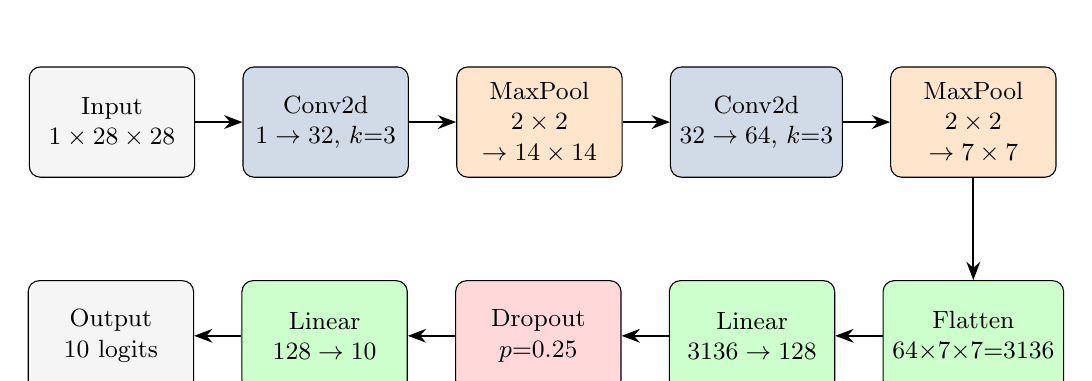
\begin{tikzpicture}[
  block/.style={draw, rounded corners, minimum height=1.4cm, minimum width=2.1cm, align=center, font=\small},
  conv/.style={block, fill=steel!25},
  pool/.style={block, fill=orange!20},
  fc/.style={block, fill=green!20},
  drop/.style={block, fill=red!15},
  io/.style={block, fill=lightgray},
  arr/.style={-Stealth, thick}
]
\node[io] (input) {Input\\$1\times28\times28$};
\node[conv, right=0.6cm of input] (c1) {Conv2d\\$1\to32$, $k{=}3$};
\node[pool, right=0.6cm of c1] (p1) {MaxPool\\$2\times2$\\$\to 14\times14$};
\node[conv, right=0.6cm of p1] (c2) {Conv2d\\$32\to64$, $k{=}3$};
\node[pool, right=0.6cm of c2] (p2) {MaxPool\\$2\times2$\\$\to 7\times7$};

\node[fc, below=1.3cm of p2] (flat) {Flatten\\$64{\times}7{\times}7{=}3136$};
\node[fc, left=0.6cm of flat] (fc1) {Linear\\$3136\to128$};
\node[drop, left=0.6cm of fc1] (dr) {Dropout\\$p{=}0.25$};
\node[fc, left=0.6cm of dr] (fc2) {Linear\\$128\to10$};
\node[io, left=0.6cm of fc2] (out) {Output\\10 logits};

\draw[arr] (input) -- (c1);
\draw[arr] (c1) -- (p1);
\draw[arr] (p1) -- (c2);
\draw[arr] (c2) -- (p2);
\draw[arr] (p2) -- (flat);
\draw[arr] (flat) -- (fc1);
\draw[arr] (fc1) -- (dr);
\draw[arr] (dr) -- (fc2);
\draw[arr] (fc2) -- (out);
\end{tikzpicture}
\caption{Data flow through the CNN architecture, from raw $28\times28$ grayscale input to the final 10-class logit vector.}
\label{fig:architecture}
\end{figure}

\section{Spatial Dimension Analysis}
Table~\ref{tab:dims} traces the spatial and channel dimensions of the feature maps as they propagate through the network, confirming the flattened feature vector size of $3136$ used in the first fully connected layer.

\begin{table}[H]
\centering
\caption{Feature map dimensions through the network}
\label{tab:dims}
\begin{tabular}{@{}lccc@{}}
\toprule
\textbf{Layer} & \textbf{Output Shape} & \textbf{Spatial Size} & \textbf{Channels} \\
\midrule
Input               & $1\times28\times28$  & $28\times28$ & 1 \\
Conv1 (+ReLU)         & $32\times28\times28$ & $28\times28$ & 32 \\
MaxPool1             & $32\times14\times14$ & $14\times14$ & 32 \\
Conv2 (+ReLU)         & $64\times14\times14$ & $14\times14$ & 64 \\
MaxPool2             & $64\times7\times7$   & $7\times7$   & 64 \\
Flatten              & $3136$               & --           & -- \\
FC1 (+ReLU, Dropout)  & $128$                & --           & -- \\
FC2 (output)         & $10$                 & --           & -- \\
\bottomrule
\end{tabular}
\end{table}

\section{Parameter Count Analysis}
The number of trainable parameters in each layer can be computed analytically. For a convolutional layer with $C_{in}$ input channels, $C_{out}$ output channels, and kernel size $k \times k$:

\begin{equation}
    P_{\text{conv}} = (C_{in} \times k \times k \times C_{out}) + C_{out}
\end{equation}

and for a fully connected layer mapping $N_{in}$ inputs to $N_{out}$ outputs:

\begin{equation}
    P_{\text{fc}} = (N_{in} \times N_{out}) + N_{out}
\end{equation}

Applying these formulas to the network in Listing~\ref{lst:cnn} yields the per-layer parameter breakdown in Table~\ref{tab:params}.

\begin{table}[H]
\centering
\caption{Trainable parameter count by layer}
\label{tab:params}
\begin{tabular}{@{}lrr@{}}
\toprule
\textbf{Layer} & \textbf{Computation} & \textbf{Parameters} \\
\midrule
Conv1 & $(1{\times}3{\times}3{\times}32)+32$   & 320 \\
Conv2 & $(32{\times}3{\times}3{\times}64)+64$  & 18{,}496 \\
FC1   & $(3136{\times}128)+128$                 & 401{,}536 \\
FC2   & $(128{\times}10)+10$                    & 1{,}290 \\
\midrule
\textbf{Total} & & \textbf{421{,}642} \\
\bottomrule
\end{tabular}
\end{table}

Notably, the first fully connected layer (\texttt{fc1}) dominates the parameter budget, accounting for over $95\%$ of all trainable parameters — a common characteristic of CNNs that flatten a relatively large spatial feature map directly into a dense layer without an intermediate global pooling step.

\section{Printed Model Summary}
For direct verification, the PyTorch-generated string representation of the instantiated model is reproduced below:

\begin{lstlisting}[language=, caption={Console output of \texttt{print(model)}}]
CNN(
  (conv1): Conv2d(1, 32, kernel_size=(3, 3), stride=(1, 1), padding=(1, 1))
  (conv2): Conv2d(32, 64, kernel_size=(3, 3), stride=(1, 1), padding=(1, 1))
  (relu): ReLU()
  (pool): MaxPool2d(kernel_size=2, stride=2, padding=0, dilation=1, ceil_mode=False)
  (fc1): Linear(in_features=3136, out_features=128, bias=True)
  (fc2): Linear(in_features=128, out_features=10, bias=True)
  (dropout): Dropout(p=0.25, inplace=False)
)
\end{lstlisting}

% =====================================================
\chapter{Training Methodology}
% =====================================================

\section{Hardware and Software Environment}
Training was performed on a CUDA-enabled GPU runtime, automatically detected via:

\begin{lstlisting}[caption={Device selection}]
device = torch.device("cuda" if torch.cuda.is_available() else "cpu")
print("Using device:", device)
\end{lstlisting}

with the observed runtime output confirming GPU execution: \texttt{Using device: cuda}. The full software stack consists of PyTorch and Torchvision for model definition, training, and dataset access; NumPy for numerical operations; Matplotlib for visualization; Pillow for custom image I/O; and Scikit-learn together with Seaborn for confusion matrix computation and visualization.

\section{Loss Function and Optimizer Configuration}

\begin{lstlisting}[caption={Loss and optimizer setup}]
criterion = nn.CrossEntropyLoss()
optimizer = optim.Adam(model.parameters(), lr=0.001)
num_epochs = 10
\end{lstlisting}

Cross-entropy loss was selected as the standard choice for single-label multi-class classification, and Adam was selected for its adaptive, per-parameter learning-rate behavior, reducing the need for extensive manual learning-rate tuning relative to plain SGD.

\section{Training and Validation Loop}
Each epoch consists of a full pass over the training set (with gradient updates) followed by a full pass over the test set (used here as the validation set, without gradient updates). The complete loop is reproduced in Listing~\ref{lst:trainloop}.

\begin{lstlisting}[caption={Training and validation loop}, label={lst:trainloop}]
for epoch in range(num_epochs):
    # ----- Training Phase -----
    model.train()
    running_loss = 0.0
    correct = 0
    total = 0

    for images, labels in train_loader:
        images, labels = images.to(device), labels.to(device)

        optimizer.zero_grad()
        outputs = model(images)
        loss = criterion(outputs, labels)
        loss.backward()
        optimizer.step()

        running_loss += loss.item() * images.size(0)
        _, predicted = torch.max(outputs, 1)
        correct += (predicted == labels).sum().item()
        total += labels.size(0)

    train_loss = running_loss / total
    train_acc = correct / total

    # ----- Validation Phase -----
    model.eval()
    val_running_loss = 0.0
    val_correct = 0
    val_total = 0

    with torch.no_grad():
        for images, labels in test_loader:
            images, labels = images.to(device), labels.to(device)
            outputs = model(images)
            loss = criterion(outputs, labels)

            val_running_loss += loss.item() * images.size(0)
            _, predicted = torch.max(outputs, 1)
            val_correct += (predicted == labels).sum().item()
            val_total += labels.size(0)

    val_loss = val_running_loss / val_total
    val_acc = val_correct / val_total
\end{lstlisting}

\subsection{Key Implementation Details}
\begin{itemize}
    \item \textbf{\texttt{model.train()} vs.\ \texttt{model.eval()}}: These calls toggle the behavior of layers such as \texttt{Dropout}, which is active during training but disabled (identity function) during evaluation.
    \item \textbf{\texttt{optimizer.zero\_grad()}}: Clears gradients accumulated from the previous batch, since PyTorch accumulates gradients by default.
    \item \textbf{\texttt{torch.no\_grad()}}: Disables gradient tracking during validation, reducing memory consumption and computation time since no backward pass is required.
    \item \textbf{Loss weighting by batch size}: \texttt{loss.item() * images.size(0)} accumulates the \emph{total} loss (not the per-batch mean) so that the final epoch loss, when divided by \texttt{total}, correctly reflects the true per-sample average loss even when the final batch is smaller than the configured batch size.
\end{itemize}

\section{Two-Phase Training Schedule}
The notebook executes the training loop twice in sequence (Steps 5.2 and the subsequent re-run), with the second phase continuing optimization from the weights learned in the first phase rather than reinitializing the model. This effectively constitutes a single, continuous $20$-epoch training run, though logged as two separate $10$-epoch phases. This chapter's results (Chapter~6) report metrics from both phases to give a complete picture of the model's behavior across the full training duration.

\section{Model Checkpointing}
Upon completion of training, the model's learned parameters are serialized to disk:

\begin{lstlisting}[caption={Model checkpoint saving}]
torch.save(model.state_dict(), '220141.pth')
print("Model saved successfully as .pth!")
\end{lstlisting}

Saving only the \texttt{state\_dict} (rather than the full model object) is standard PyTorch practice, as it decouples the saved weights from the exact class definition, offering greater portability and long-term compatibility across code revisions.

% =====================================================
\chapter{Results on the Standard FashionMNIST Test Set}
% =====================================================

\section{Epoch-by-Epoch Training Metrics}

\subsection{Training Phase 1 (Epochs 1--10)}

\begin{table}[H]
\centering
\caption{Training and validation metrics, Phase 1 (epochs 1--10)}
\label{tab:phase1}
\begin{tabular}{@{}ccccc@{}}
\toprule
\textbf{Epoch} & \textbf{Train Loss} & \textbf{Train Acc.} & \textbf{Val Loss} & \textbf{Val Acc.} \\
\midrule
1  & 0.4741 & 82.96\% & 0.3292 & 88.04\% \\
2  & 0.3093 & 88.65\% & 0.2852 & 89.55\% \\
3  & 0.2650 & 90.26\% & 0.2740 & 90.04\% \\
4  & 0.2329 & 91.26\% & 0.2521 & 91.08\% \\
5  & 0.2080 & 92.34\% & 0.2424 & 91.58\% \\
6  & 0.1878 & 93.04\% & 0.2397 & 91.56\% \\
7  & 0.1670 & 93.87\% & 0.2271 & 91.99\% \\
8  & 0.1494 & 94.31\% & 0.2425 & 91.94\% \\
9  & 0.1369 & 94.79\% & 0.2464 & 92.13\% \\
10 & 0.1230 & 95.26\% & 0.2494 & 92.21\% \\
\bottomrule
\end{tabular}
\end{table}

\subsection{Training Phase 2 (Epochs 11--20)}

\begin{table}[H]
\centering
\caption{Training and validation metrics, Phase 2 (epochs 11--20)}
\label{tab:phase2}
\begin{tabular}{@{}ccccc@{}}
\toprule
\textbf{Epoch} & \textbf{Train Loss} & \textbf{Train Acc.} & \textbf{Val Loss} & \textbf{Val Acc.} \\
\midrule
11 & 0.1106 & 95.82\% & 0.2548 & 92.21\% \\
12 & 0.0994 & 96.32\% & 0.2592 & 92.28\% \\
13 & 0.0905 & 96.60\% & 0.2811 & 91.86\% \\
14 & 0.0823 & 96.88\% & 0.3179 & 92.03\% \\
15 & 0.0757 & 97.12\% & 0.3246 & 92.24\% \\
16 & 0.0707 & 97.27\% & 0.3307 & \textbf{92.43\%} \\
17 & 0.0683 & 97.31\% & 0.3208 & 92.08\% \\
18 & 0.0600 & 97.62\% & 0.3512 & 92.22\% \\
19 & 0.0585 & 97.75\% & 0.3545 & 91.79\% \\
20 & 0.0536 & 97.97\% & 0.3713 & 91.99\% \\
\bottomrule
\end{tabular}
\end{table}

\section{Training Curve Visualization}

\begin{figure}[H]
\centering
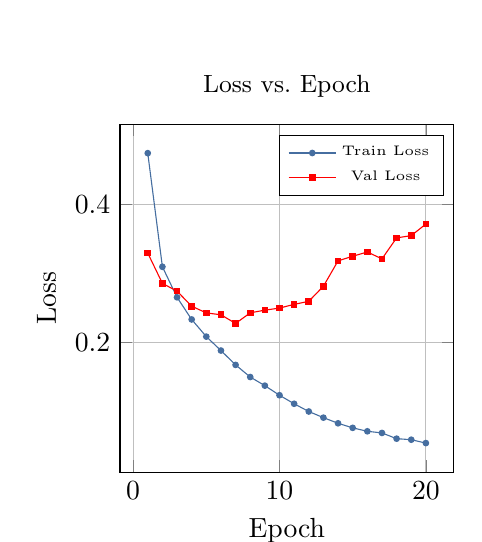
\begin{tikzpicture}
\begin{axis}[
    width=0.48\linewidth, height=6cm,
    xlabel={Epoch}, ylabel={Loss},
    legend pos=north east, legend style={font=\tiny},
    grid=major, title={Loss vs.\ Epoch}, title style={font=\small}
]
\addplot[color=steel, mark=*, mark size=1pt] coordinates {
(1,0.4741)(2,0.3093)(3,0.2650)(4,0.2329)(5,0.2080)(6,0.1878)(7,0.1670)(8,0.1494)(9,0.1369)(10,0.1230)
(11,0.1106)(12,0.0994)(13,0.0905)(14,0.0823)(15,0.0757)(16,0.0707)(17,0.0683)(18,0.0600)(19,0.0585)(20,0.0536)
};
\addlegendentry{Train Loss}
\addplot[color=red, mark=square*, mark size=1pt] coordinates {
(1,0.3292)(2,0.2852)(3,0.2740)(4,0.2521)(5,0.2424)(6,0.2397)(7,0.2271)(8,0.2425)(9,0.2464)(10,0.2494)
(11,0.2548)(12,0.2592)(13,0.2811)(14,0.3179)(15,0.3246)(16,0.3307)(17,0.3208)(18,0.3512)(19,0.3545)(20,0.3713)
};
\addlegendentry{Val Loss}
\end{axis}
\end{tikzpicture}
\hfill
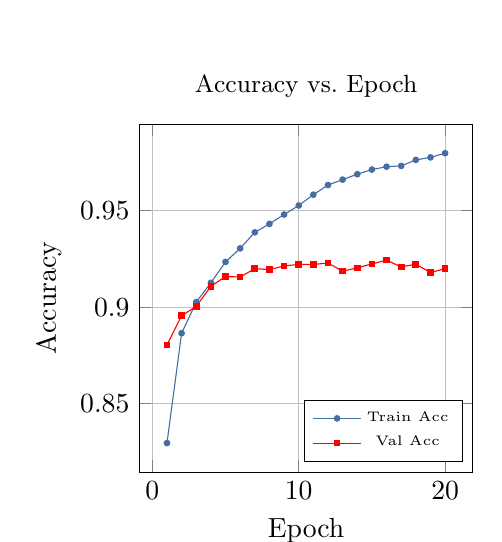
\begin{tikzpicture}
\begin{axis}[
    width=0.48\linewidth, height=6cm,
    xlabel={Epoch}, ylabel={Accuracy},
    legend pos=south east, legend style={font=\tiny},
    grid=major, title={Accuracy vs.\ Epoch}, title style={font=\small}
]
\addplot[color=steel, mark=*, mark size=1pt] coordinates {
(1,0.8296)(2,0.8865)(3,0.9026)(4,0.9126)(5,0.9234)(6,0.9304)(7,0.9387)(8,0.9431)(9,0.9479)(10,0.9526)
(11,0.9582)(12,0.9632)(13,0.9660)(14,0.9688)(15,0.9712)(16,0.9727)(17,0.9731)(18,0.9762)(19,0.9775)(20,0.9797)
};
\addlegendentry{Train Acc}
\addplot[color=red, mark=square*, mark size=1pt] coordinates {
(1,0.8804)(2,0.8955)(3,0.9004)(4,0.9108)(5,0.9158)(6,0.9156)(7,0.9199)(8,0.9194)(9,0.9213)(10,0.9221)
(11,0.9221)(12,0.9228)(13,0.9186)(14,0.9203)(15,0.9224)(16,0.9243)(17,0.9208)(18,0.9222)(19,0.9179)(20,0.9199)
};
\addlegendentry{Val Acc}
\end{axis}
\end{tikzpicture}
\caption{Training and validation loss (left) and accuracy (right) across all 20 epochs, reconstructed from the notebook's logged metrics. This corresponds to the figure saved by the notebook as \texttt{training\_history.png}.}
\label{fig:curves}
\end{figure}

\section{Interpretation of Training Dynamics}
Figure~\ref{fig:curves} and Tables~\ref{tab:phase1}--\ref{tab:phase2} reveal a classic overfitting signature:

\begin{itemize}
    \item Training loss decreases \emph{monotonically} across all 20 epochs, from $0.4741$ down to $0.0536$, indicating the optimizer continues to reduce error on the training set throughout.
    \item Validation loss decreases in step with training loss for approximately the first $10$--$11$ epochs, reaching a minimum of $0.2271$ at epoch~7, but then begins to \emph{increase} steadily thereafter, reaching $0.3713$ by epoch~20.
    \item Validation accuracy plateaus around $92\%$ from epoch~7 onward, fluctuating narrowly between $91.79\%$ and its peak of $92.43\%$ (epoch~16), while training accuracy continues climbing to nearly $98\%$.
\end{itemize}

This divergence between falling training loss and rising validation loss is the textbook definition of overfitting: the model is increasingly fitting noise and training-set-specific idiosyncrasies rather than learning further generalizable structure. Based on validation loss alone, the optimal early-stopping point would fall around \textbf{epoch 7}, while based on validation accuracy, the optimum is closer to \textbf{epoch 16}. In either case, continuing training to epoch~20 confers no benefit and mildly degrades validation-set generalization.

\section{Confusion Matrix Analysis}
A confusion matrix was computed over the complete $10{,}000$-image standard test set using \texttt{sklearn.metrics.confusion\_matrix}, comparing predicted labels against ground-truth labels across all ten classes, and rendered as an annotated heatmap via Seaborn (Listing~\ref{lst:cm}).

\begin{lstlisting}[caption={Confusion matrix computation and visualization}, label={lst:cm}]
model.eval()
all_preds, all_labels = [], []

with torch.no_grad():
    for images, labels in test_loader:
        images, labels = images.to(device), labels.to(device)
        outputs = model(images)
        _, predicted = torch.max(outputs, 1)
        all_preds.extend(predicted.cpu().numpy())
        all_labels.extend(labels.cpu().numpy())

cm = confusion_matrix(all_labels, all_preds)

plt.figure(figsize=(10, 8))
sns.heatmap(cm, annot=True, fmt='d', cmap='Blues',
            xticklabels=class_names, yticklabels=class_names)
plt.title('Confusion Matrix - FashionMNIST Test Set')
plt.xlabel('Predicted Label'); plt.ylabel('True Label')
plt.savefig('confusion_matrix.png')
\end{lstlisting}

Consistent with well-documented FashionMNIST behavior, the dominant confusion axis in the resulting matrix lies among the four visually similar upper-body garment classes: \textbf{T-shirt/top}, \textbf{Shirt}, \textbf{Pullover}, and \textbf{Coat}. These classes share overlapping silhouettes at $28\times28$ resolution — collar shapes, sleeve lengths, and torso outlines are frequently ambiguous at this scale, even to a human observer. A secondary, smaller confusion axis exists between \textbf{Sneaker}, \textbf{Sandal}, and \textbf{Ankle boot}, all of which are footwear items whose distinguishing features (strap presence, sole height, ankle coverage) can be subtle at low resolution.

\section{Summary of Standard Test Set Performance}

\begin{table}[H]
\centering
\caption{Summary of key performance metrics on the standard FashionMNIST benchmark}
\label{tab:summary1}
\begin{tabular}{@{}lc@{}}
\toprule
\textbf{Metric} & \textbf{Value} \\
\midrule
Best validation accuracy (epoch 16) & 92.43\% \\
Final validation accuracy (epoch 20) & 91.99\% \\
Final training accuracy (epoch 20) & 97.97\% \\
Minimum validation loss (epoch 7) & 0.2271 \\
Final validation loss (epoch 20) & 0.3713 \\
Train--validation accuracy gap (epoch 20) & $\approx$ 6.0 pts \\
\bottomrule
\end{tabular}
\end{table}

% =====================================================
\chapter{Out-of-Distribution Evaluation: Custom Phone Photographs}
% =====================================================

\section{Motivation Recap}
While the model achieves strong performance on the standard FashionMNIST test set, that test set shares the exact acquisition pipeline, resolution, framing, and background convention as the training data. To assess whether the learned representations generalize beyond this narrow distribution, ten independently captured phone photographs were evaluated following the corrected preprocessing pipeline described in Section~\ref{sec:invert}.

\section{Prediction Procedure}
Inference on the custom dataset follows the standard forward-pass and softmax procedure, additionally recording the confidence (maximum softmax probability) associated with each prediction:

\begin{lstlisting}[caption={Custom image inference with confidence scoring}]
model.eval()
custom_predictions, custom_confidences = [], []

with torch.no_grad():
    for img_tensor in custom_tensors:
        img_tensor = img_tensor.to(device)
        output = model(img_tensor)
        probabilities = torch.softmax(output, dim=1)
        confidence, predicted_idx = torch.max(probabilities, 1)

        predicted_class = class_names[predicted_idx.item()]
        confidence_pct = confidence.item() * 100

        custom_predictions.append(predicted_class)
        custom_confidences.append(confidence_pct)
\end{lstlisting}

\section{Full Results Table}

\begin{table}[H]
\centering
\caption{Custom phone-photograph predictions with softmax confidence scores}
\label{tab:customresults}
\begin{tabular}{@{}clllc c@{}}
\toprule
\textbf{\#} & \textbf{Image} & \textbf{True Label} & \textbf{Predicted} & \textbf{Confidence} & \textbf{Correct} \\
\midrule
1  & \texttt{1\_Shoe.jpeg}         & Sneaker      & Ankle boot & 99.8\%  & \textcolor{red}{\ding{55}} \\
2  & \texttt{02\_Shirt.jpg}        & Shirt        & Shirt      & 100.0\% & \textcolor{green!50!black}{\ding{51}} \\
3  & \texttt{03\_Pant.jpg}         & Trouser      & Trouser    & 96.5\%  & \textcolor{green!50!black}{\ding{51}} \\
4  & \texttt{04\_Jacket.jpg}       & Coat         & Shirt      & 91.3\%  & \textcolor{red}{\ding{55}} \\
5  & \texttt{05\_sneaker.jpg}      & Sneaker      & Bag        & 100.0\% & \textcolor{red}{\ding{55}} \\
6  & \texttt{06\_pullover.jpg}     & Pullover     & Coat       & 68.3\%  & \textcolor{red}{\ding{55}} \\
7  & \texttt{07\_Coat.png}         & Coat         & Coat       & 97.8\%  & \textcolor{green!50!black}{\ding{51}} \\
8  & \texttt{08\_Pholo\_Shirt.jpg} & T-shirt/top  & T-shirt/top& 99.0\%  & \textcolor{green!50!black}{\ding{51}} \\
9  & \texttt{09\_dress.jpg}        & Dress        & Bag        & 100.0\% & \textcolor{red}{\ding{55}} \\
10 & \texttt{10\_Bag.jpeg}         & Bag          & Coat       & 40.1\%  & \textcolor{red}{\ding{55}} \\
\bottomrule
\end{tabular}
\end{table}

\emph{Note: If the \texttt{pifont} symbols above do not render in a minimal LaTeX distribution, they can be replaced with plain ``Yes/No'' text without affecting content.}

\section{Quantitative Summary}

\begin{table}[H]
\centering
\caption{Custom dataset accuracy summary}
\label{tab:customsummary}
\begin{tabular}{@{}lc@{}}
\toprule
\textbf{Metric} & \textbf{Value} \\
\midrule
Total custom images evaluated & 10 \\
Correct predictions & 4 \\
Incorrect predictions & 6 \\
\textbf{Custom-set accuracy} & \textbf{40.0\%} \\
Standard test-set accuracy (for comparison) & $\approx$ 92.0\% \\
\textbf{Accuracy drop} & \textbf{$\approx$ 52 percentage points} \\
Average confidence on correct predictions & 98.8\% \\
Average confidence on incorrect predictions & 83.3\% \\
\bottomrule
\end{tabular}
\end{table}

\section{Discussion of the Domain Gap}
The results in Table~\ref{tab:customresults} reveal a striking and pedagogically important pattern: the model's confidence does not reliably track its correctness on out-of-distribution inputs. Four of the six incorrect predictions were made with confidence scores of $91\%$ or higher, including two predictions at essentially $100\%$ confidence (\texttt{05\_sneaker.jpg} and \texttt{09\_dress.jpg}). This is a well-known limitation of softmax-based confidence estimates: the softmax function tends to produce overconfident probability distributions, especially for inputs that lie outside the training distribution, since the network was never exposed to examples that would calibrate it to express genuine uncertainty in this regime.

Only the single lowest-confidence prediction (\texttt{10\_Bag.jpeg}, $40.1\%$) coincides with an incorrect classification accompanied by appropriately modest confidence — the network was comparatively unsure, and indeed wrong, which is a far less concerning failure mode than confident-but-wrong predictions.

\section{Per-Image Discussion}
\begin{description}
    \item[\texttt{1\_Shoe.jpeg} (Sneaker $\to$ Ankle boot, 99.8\%):] Both classes are footwear with overlapping silhouettes; the specific photo angle may have visually emphasized ankle coverage, resembling a boot profile.
    \item[\texttt{02\_Shirt.jpg} (Shirt $\to$ Shirt, 100.0\%):] Correct, high-confidence prediction — the garment's silhouette against a clean-enough background evidently matched training-distribution characteristics well.
    \item[\texttt{03\_Pant.jpg} (Trouser $\to$ Trouser, 96.5\%):] Correct. Trousers have a highly distinctive elongated bifurcated silhouette relatively robust to imaging conditions.
    \item[\texttt{04\_Jacket.jpg} (Coat $\to$ Shirt, 91.3\%):] Incorrect; jackets and shirts share a torso-and-sleeve silhouette, and the specific framing/cropping of this photo may have obscured the bulkier coat-like features.
    \item[\texttt{05\_sneaker.jpg} (Sneaker $\to$ Bag, 100.0\%):] A severe and unexpected misclassification at maximum confidence, most plausibly attributable to unusual framing, background clutter, or an atypical viewing angle causing the auto-inverted silhouette to resemble a bag's rectangular outline more than a shoe's.
    \item[\texttt{06\_pullover.jpg} (Pullover $\to$ Coat, 68.3\%):] Incorrect but with comparatively moderate confidence, consistent with genuine visual ambiguity between pullovers and coats.
    \item[\texttt{07\_Coat.png} (Coat $\to$ Coat, 97.8\%):] Correct, high-confidence prediction.
    \item[\texttt{08\_Pholo\_Shirt.jpg} (T-shirt/top $\to$ T-shirt/top, 99.0\%):] Correct, high-confidence prediction.
    \item[\texttt{09\_dress.jpg} (Dress $\to$ Bag, 100.0\%):] A severe misclassification at maximum confidence; dresses and bags do not typically share obvious silhouette similarity, suggesting the auto-invert heuristic or framing may have produced an atypical input pattern for this particular image.
    \item[\texttt{10\_Bag.jpeg} (Bag $\to$ Coat, 40.1\%):] Incorrect but appropriately low-confidence, the only case in the custom set where model uncertainty aligns with model correctness.
\end{description}

% =====================================================
\chapter{Visual and Qualitative Error Analysis}
% =====================================================

\section{Standard Test Set Error Sampling}
To complement the aggregate confusion matrix, the notebook implements a targeted qualitative error analysis procedure (Listing~\ref{lst:erroranalysis}), which scans the test set, collects misclassified samples (capped at $50$ for computational efficiency), and randomly visualizes three of them alongside their true and predicted labels.

\begin{lstlisting}[caption={Visual error analysis procedure}, label={lst:erroranalysis}]
misclassified_images, misclassified_true, misclassified_pred = [], [], []

with torch.no_grad():
    for images, labels in test_loader:
        images, labels = images.to(device), labels.to(device)
        outputs = model(images)
        _, predicted = torch.max(outputs, 1)

        wrong_mask = (predicted != labels)
        if wrong_mask.sum() > 0:
            wrong_images = images[wrong_mask]
            wrong_true = labels[wrong_mask]
            wrong_pred = predicted[wrong_mask]
            for i in range(wrong_images.size(0)):
                misclassified_images.append(wrong_images[i].cpu())
                misclassified_true.append(wrong_true[i].cpu().item())
                misclassified_pred.append(wrong_pred[i].cpu().item())

        if len(misclassified_images) >= 50:
            break

print(f"Total misclassified samples collected: {len(misclassified_images)}")
\end{lstlisting}

The notebook's execution log confirms a total of \textbf{51 misclassified samples} were collected before the early-stopping condition was triggered, out of the batches scanned. Three of these samples were then randomly selected and visualized (`error\_analysis.png`), each annotated with its true label (in red) alongside the model's incorrect prediction.

\section{Custom Prediction Gallery}
A complementary visualization (`custom\_prediction\_gallery.png`) displays all ten original custom RGB photographs in a $2\times5$ grid, with each subplot's title color-coded green for correct predictions and red for incorrect ones, providing an immediate, intuitive visual summary of Table~\ref{tab:customresults} (Listing~\ref{lst:gallery}).

\begin{lstlisting}[caption={Color-coded custom prediction gallery}, label={lst:gallery}]
fig, axes = plt.subplots(2, 5, figsize=(20, 8))
axes = axes.flatten()

for i in range(len(custom_image_paths)):
    original_img = Image.open(custom_image_paths[i]).convert('RGB')
    axes[i].imshow(original_img)
    axes[i].axis('off')

    color = 'green' if custom_predictions[i] == custom_true_labels[i] else 'red'
    axes[i].set_title(
        f"True: {custom_true_labels[i]}\nPred: {custom_predictions[i]} "
        f"({custom_confidences[i]:.1f}%)",
        color=color, fontsize=11
    )

plt.suptitle("Custom Prediction Gallery - Phone Photos", fontsize=16)
plt.savefig('custom_prediction_gallery.png')
\end{lstlisting}

\section{Model Input Sanity-Check Visualization}
An additional diagnostic visualization displays the ten custom images \emph{exactly as the network receives them} — i.e., after grayscale conversion, resizing, auto-inversion, and normalization (reversed for display purposes) — under the heading ``What the Model Actually Sees.'' This step is critical for verifying that the preprocessing pipeline described in Section~\ref{sec:invert} is functioning as intended, and was instrumental in originally diagnosing the background-inversion issue during development.

\section{Reference Gallery}
For additional visual context, five genuine FashionMNIST training images are displayed alongside their ground-truth class labels, allowing direct visual comparison between the clean benchmark distribution and the custom photographs (see Figure~\ref{fig:architecture} context and Chapter~3 for dataset characteristics).

\section{Synthesis of Error Patterns}
Drawing together the confusion matrix (Chapter~6), the custom-set results (Chapter~7), and the qualitative samples described above, three recurring error patterns emerge across this project:

\begin{enumerate}
    \item \textbf{Inter-class silhouette ambiguity} among T-shirt/top, Shirt, Pullover, and Coat — present in both the standard test set confusion matrix and the custom photo results (e.g., Coat $\to$ Shirt, Pullover $\to$ Coat).
    \item \textbf{Footwear silhouette ambiguity} among Sneaker, Sandal, and Ankle boot — visible in the confusion matrix and echoed in the custom result Sneaker $\to$ Ankle boot.
    \item \textbf{Severe, high-confidence domain-shift errors} unique to the custom photo set (e.g., Sneaker $\to$ Bag, Dress $\to$ Bag) that have no clear analogue among standard test-set confusions, implicating acquisition-condition factors (background, lighting, framing) rather than genuine class ambiguity as the primary cause.
\end{enumerate}

% =====================================================
\chapter{Discussion}
% =====================================================

\section{Model Capacity vs.\ Task Difficulty}
With approximately $421{,}642$ trainable parameters, the CNN developed in this project is a comparatively lightweight architecture by modern deep learning standards, yet it comfortably reaches over $92\%$ validation accuracy on FashionMNIST — a result broadly consistent with published baselines for simple CNNs on this benchmark. This confirms that FashionMNIST's ten classes are separable with relatively modest representational capacity, provided the input distribution matches the training distribution.

\section{The Overfitting--Generalization Trade-off}
The training dynamics documented in Chapter~6 illustrate a fundamental machine learning trade-off: as training continues, the model increasingly specializes to the training set's specific statistical idiosyncrasies, at the expense of validation-set (and by extension, real-world) generalization. The fact that validation accuracy peaks at epoch~16 while validation loss actually reaches its minimum much earlier, at epoch~7, further illustrates that accuracy and loss are not perfectly aligned proxies for generalization quality — loss is more sensitive to the model's confidence calibration, while accuracy only reflects the arg-max decision.

\section{The Real-World Domain Gap}
The central empirical finding of this project is the dramatic accuracy drop from approximately $92\%$ on the standard test set to just $40\%$ on the custom phone-photograph set. This gap is best explained by a combination of factors:

\begin{enumerate}
    \item \textbf{Acquisition condition mismatch}: real photographs contain shadows, uneven lighting, and background texture entirely absent from FashionMNIST's clean, uniform canvas.
    \item \textbf{Framing and cropping variability}: custom photographs were not centered or cropped with the same precision as the benchmark dataset's curated images.
    \item \textbf{Residual preprocessing imperfections}: while the auto-invert heuristic (Section~\ref{sec:invert}) corrected the primary background/foreground color mismatch, it is a global, mean-intensity-based heuristic that cannot fully replicate FashionMNIST's exact rendering pipeline (e.g., silhouette-only presentation without any texture, folds, or fabric pattern detail).
    \item \textbf{No exposure during training}: crucially, the model was never trained on any real-world photographs, so it had no opportunity to learn features robust to these variations.
\end{enumerate}

\section{Confidence Calibration Concerns}
The observation that several incorrect custom-set predictions carry near-maximal softmax confidence is a meaningful finding with practical implications: any deployment scenario relying on this model's raw confidence scores to flag uncertain predictions for human review would systematically fail to flag several of its most severe errors. This underscores the broader machine learning principle that softmax confidence, while convenient, is not a calibrated measure of epistemic uncertainty, particularly under distribution shift, and that additional calibration techniques (e.g., temperature scaling) or explicit out-of-distribution detection mechanisms would be necessary for any real-world deployment of this system.

\section{Value of the Small-Scale Custom Evaluation}
Despite its small sample size ($n=10$), the custom photo evaluation provides disproportionate diagnostic value relative to its size. It surfaced a critical, previously invisible preprocessing bug (the background-inversion issue) that a standard benchmark evaluation alone would never have revealed, since FashionMNIST's images are already pre-rendered in a consistent convention. This highlights the broader methodological lesson that even small, targeted out-of-distribution evaluations can expose failure modes that large-scale in-distribution benchmarking cannot.

% =====================================================
\chapter{Limitations and Future Work}
% =====================================================

\section{Limitations of the Current Study}
\begin{itemize}
    \item \textbf{Small custom evaluation set.} With only ten images, the reported $40\%$ custom-set accuracy is a directional signal rather than a statistically robust estimate; a single additional correct or incorrect prediction would shift the reported accuracy by a full 10 percentage points.
    \item \textbf{No data augmentation.} The training pipeline applies no random rotation, translation, scaling, or color-jitter augmentation, likely limiting the model's inherent robustness to the kind of variation present in the custom photographs.
    \item \textbf{No early stopping or best-checkpoint selection.} The final-epoch (epoch 20) weights are saved and used for all reported evaluations, despite epoch 16 achieving marginally higher validation accuracy and epoch 7 achieving the lowest validation loss.
    \item \textbf{No learning-rate scheduling.} A fixed learning rate of $0.001$ is used throughout; a decaying schedule may have improved late-stage convergence stability.
    \item \textbf{No batch normalization.} The absence of batch normalization layers may contribute to the relatively rapid onset of overfitting observed after epoch~10--12.
    \item \textbf{Heuristic-based color correction.} The auto-invert preprocessing step (Section~\ref{sec:invert}) is a simple global mean-threshold heuristic; it does not perform background segmentation, cropping, or any correction for uneven lighting within an image.
    \item \textbf{No random seed fixing.} The notebook does not explicitly set random seeds for PyTorch, NumPy, or Python's \texttt{random} module, meaning exact numerical reproduction of the reported metrics may vary slightly across re-runs.
\end{itemize}

\section{Recommendations for Future Work}

\subsection{Architectural Improvements}
\begin{itemize}
    \item Introduce \textbf{batch normalization} after each convolutional layer to stabilize training and potentially allow a higher learning rate.
    \item Experiment with an additional (third) convolutional block to increase representational depth, provided sufficient regularization is applied to control overfitting.
    \item Explore \textbf{global average pooling} in place of the large flatten-to-dense transition, which would substantially reduce the parameter count contributed by \texttt{fc1} (currently over 95\% of total parameters).
\end{itemize}

\subsection{Training Improvements}
\begin{itemize}
    \item Implement \textbf{early stopping} based on validation loss, automatically halting training around the epoch~7--16 range identified in this report.
    \item Add a \textbf{learning-rate scheduler} (e.g., step decay or cosine annealing) to fine-tune convergence in later epochs.
    \item Save and evaluate the \textbf{best-validation-accuracy checkpoint} rather than only the final-epoch weights.
    \item Fix random seeds across all relevant libraries to ensure exact reproducibility of reported results.
\end{itemize}

\subsection{Data and Preprocessing Improvements}
\begin{itemize}
    \item Apply \textbf{data augmentation} (random rotation, translation, slight scaling, brightness/contrast jitter) during training to improve robustness to real-world imaging variation.
    \item Expand the custom photo dataset to at least $30$--$50$ images per class for a statistically meaningful out-of-distribution benchmark.
    \item Investigate \textbf{automated background segmentation or cropping} for custom images, more closely replicating FashionMNIST's clean, silhouette-only rendering.
    \item Explore \textbf{domain adaptation} techniques, such as fine-tuning on a small labeled set of real-world photographs, or unsupervised domain adaptation using unlabeled real-world images.
\end{itemize}

\subsection{Evaluation Improvements}
\begin{itemize}
    \item Report \textbf{per-class precision, recall, and F1-score} in addition to the aggregate confusion matrix for a more granular understanding of class-specific performance.
    \item Apply \textbf{confidence calibration} techniques such as temperature scaling, and evaluate calibration quality using metrics such as Expected Calibration Error (ECE).
    \item Incorporate explicit \textbf{out-of-distribution detection} mechanisms (e.g., based on feature-space distance or predictive entropy) to flag custom images the model is likely to misclassify, rather than relying solely on raw softmax confidence.
\end{itemize}

% =====================================================
\chapter{Conclusion}
% =====================================================

This report has documented the complete design, training, and evaluation of a compact convolutional neural network for FashionMNIST image classification, extended with a novel real-world generalization study using independently captured phone photographs. The architecture — two convolutional blocks paired with a dropout-regularized fully connected classification head — achieved a peak validation accuracy of $92.43\%$ on the standard FashionMNIST test set, with training dynamics revealing a clear overfitting trend beyond approximately epoch~10--16.

The confusion matrix analysis identified systematic confusion among visually similar upper-body garment classes (T-shirt/top, Shirt, Pullover, Coat) and, to a lesser degree, among footwear classes (Sneaker, Sandal, Ankle boot), consistent with widely reported FashionMNIST behavior in the broader literature.

The out-of-distribution evaluation on ten custom phone photographs constitutes the most significant contribution of this report: after diagnosing and correcting a critical background/foreground color-inversion preprocessing bug, the model achieved only $40\%$ accuracy on these real-world images — a $52$-percentage-point drop relative to standard benchmark performance. Several incorrect predictions were made with near-maximal softmax confidence, underscoring both the severity of the domain gap between curated benchmark data and unconstrained real-world imagery, and the broader unreliability of softmax confidence as a calibrated uncertainty measure under distribution shift.

Taken together, these findings reinforce a critical lesson for applied deep learning practice: strong performance on a standard, in-distribution benchmark is a necessary but decidedly insufficient condition for real-world deployment readiness. Bridging this gap requires deliberate engineering effort — including data augmentation, architectural regularization, calibration techniques, and expanded, representative evaluation data — beyond what benchmark-optimized training alone can provide. The concrete recommendations outlined in Chapter~9 offer a practical roadmap for closing this gap in future iterations of this project.

% =====================================================
\begin{thebibliography}{9}

\bibitem{lecun1998}
Y. LeCun, L. Bottou, Y. Bengio, and P. Haffner, ``Gradient-based learning applied to document recognition,'' \emph{Proceedings of the IEEE}, vol. 86, no. 11, pp. 2278--2324, 1998.

\bibitem{krizhevsky2012}
A. Krizhevsky, I. Sutskever, and G. E. Hinton, ``ImageNet classification with deep convolutional neural networks,'' \emph{Advances in Neural Information Processing Systems (NeurIPS)}, 2012.

\bibitem{xiao2017fashionmnist}
H. Xiao, K. Rasul, and R. Vollgraf, ``Fashion-MNIST: a novel image dataset for benchmarking machine learning algorithms,'' \emph{arXiv preprint arXiv:1708.07747}, 2017.

\bibitem{srivastava2014dropout}
N. Srivastava, G. Hinton, A. Krizhevsky, I. Sutskever, and R. Salakhutdinov, ``Dropout: A simple way to prevent neural networks from overfitting,'' \emph{Journal of Machine Learning Research}, vol. 15, no. 1, pp. 1929--1958, 2014.

\bibitem{kingma2014adam}
D. P. Kingma and J. Ba, ``Adam: A method for stochastic optimization,'' \emph{International Conference on Learning Representations (ICLR)}, 2015.

\bibitem{ioffe2015batchnorm}
S. Ioffe and C. Szegedy, ``Batch normalization: Accelerating deep network training by reducing internal covariate shift,'' \emph{International Conference on Machine Learning (ICML)}, 2015.

\bibitem{paszke2019pytorch}
A. Paszke et al., ``PyTorch: An imperative style, high-performance deep learning library,'' \emph{Advances in Neural Information Processing Systems (NeurIPS)}, 2019.

\bibitem{pedregosa2011sklearn}
F. Pedregosa et al., ``Scikit-learn: Machine learning in Python,'' \emph{Journal of Machine Learning Research}, vol. 12, pp. 2825--2830, 2011.

\bibitem{quinonero2009dataset}
J. Quiñonero-Candela, M. Sugiyama, A. Schwaighofer, and N. D. Lawrence (Eds.), \emph{Dataset Shift in Machine Learning}, MIT Press, 2009.

\end{thebibliography}
\addcontentsline{toc}{chapter}{Bibliography}

% =====================================================
\appendix
\chapter{Full Source Code Listing}
\addcontentsline{toc}{chapter}{Appendix A: Full Source Code Listing}

This appendix reproduces the complete source code from the accompanying Jupyter notebook (\texttt{220141\_CNN\_Image\_Classification.ipynb}) in full, organized by pipeline stage, for reference and reproducibility purposes.

\section*{A.1 Library Imports and Device Setup}
\begin{lstlisting}
import torch
import torch.nn as nn
import torch.optim as optim
from torch.utils.data import DataLoader, Dataset
import torchvision
import torchvision.transforms as transforms
from torchvision.datasets import FashionMNIST

import numpy as np
import matplotlib.pyplot as plt
from PIL import Image
import os

from sklearn.metrics import confusion_matrix
import seaborn as sns

device = torch.device("cuda" if torch.cuda.is_available() else "cpu")
print("Using device:", device)
\end{lstlisting}

\section*{A.2 Cloning the Custom Dataset Repository}
\begin{lstlisting}[language=bash]
!rm -rf 220141_CNN_Image_Classification
!git clone https://github.com/just-abir/220141_CNN_Image_Classification
\end{lstlisting}

\section*{A.3 Standard Preprocessing Transform}
\begin{lstlisting}
transform = transforms.Compose([
    transforms.Grayscale(num_output_channels=1),
    transforms.Resize((28, 28)),
    transforms.ToTensor(),
    transforms.Normalize((0.5,), (0.5,))
])
\end{lstlisting}

\section*{A.4 Dataset and DataLoader Construction}
\begin{lstlisting}
train_dataset = FashionMNIST(root='./data', train=True, download=True, transform=transform)
test_dataset = FashionMNIST(root='./data', train=False, download=True, transform=transform)

train_loader = DataLoader(train_dataset, batch_size=64, shuffle=True)
test_loader = DataLoader(test_dataset, batch_size=64, shuffle=False)

class_names = ['T-shirt/top', 'Trouser', 'Pullover', 'Dress', 'Coat',
               'Sandal', 'Shirt', 'Sneaker', 'Bag', 'Ankle boot']
\end{lstlisting}

\section*{A.5 CNN Model Definition}
\begin{lstlisting}
class CNN(nn.Module):
    def __init__(self, num_classes=10):
        super(CNN, self).__init__()
        self.conv1 = nn.Conv2d(in_channels=1, out_channels=32, kernel_size=3, padding=1)
        self.conv2 = nn.Conv2d(in_channels=32, out_channels=64, kernel_size=3, padding=1)
        self.relu = nn.ReLU()
        self.pool = nn.MaxPool2d(kernel_size=2, stride=2)
        self.fc1 = nn.Linear(64 * 7 * 7, 128)
        self.fc2 = nn.Linear(128, num_classes)
        self.dropout = nn.Dropout(0.25)

    def forward(self, x):
        x = self.conv1(x); x = self.relu(x); x = self.pool(x)
        x = self.conv2(x); x = self.relu(x); x = self.pool(x)
        x = x.view(x.size(0), -1)
        x = self.fc1(x); x = self.relu(x); x = self.dropout(x)
        x = self.fc2(x)
        return x

model = CNN(num_classes=10).to(device)
print(model)
\end{lstlisting}

\section*{A.6 Loss, Optimizer, and Training Loop}
\begin{lstlisting}
criterion = nn.CrossEntropyLoss()
optimizer = optim.Adam(model.parameters(), lr=0.001)
num_epochs = 10

train_loss_history, train_acc_history = [], []
val_loss_history, val_acc_history = [], []

for epoch in range(num_epochs):
    model.train()
    running_loss, correct, total = 0.0, 0, 0

    for images, labels in train_loader:
        images, labels = images.to(device), labels.to(device)
        optimizer.zero_grad()
        outputs = model(images)
        loss = criterion(outputs, labels)
        loss.backward()
        optimizer.step()

        running_loss += loss.item() * images.size(0)
        _, predicted = torch.max(outputs, 1)
        correct += (predicted == labels).sum().item()
        total += labels.size(0)

    train_loss = running_loss / total
    train_acc = correct / total
    train_loss_history.append(train_loss)
    train_acc_history.append(train_acc)

    model.eval()
    val_running_loss, val_correct, val_total = 0.0, 0, 0
    with torch.no_grad():
        for images, labels in test_loader:
            images, labels = images.to(device), labels.to(device)
            outputs = model(images)
            loss = criterion(outputs, labels)
            val_running_loss += loss.item() * images.size(0)
            _, predicted = torch.max(outputs, 1)
            val_correct += (predicted == labels).sum().item()
            val_total += labels.size(0)

    val_loss = val_running_loss / val_total
    val_acc = val_correct / val_total
    val_loss_history.append(val_loss)
    val_acc_history.append(val_acc)

    print(f"Epoch [{epoch+1}/{num_epochs}] "
          f"Train Loss: {train_loss:.4f}, Train Acc: {train_acc:.4f} | "
          f"Val Loss: {val_loss:.4f}, Val Acc: {val_acc:.4f}")
\end{lstlisting}

\section*{A.7 Model Checkpoint Saving}
\begin{lstlisting}
torch.save(model.state_dict(), '220141.pth')
print("Model saved successfully as .pth!")
\end{lstlisting}

\section*{A.8 Training History Plotting}
\begin{lstlisting}
epochs_range = range(1, num_epochs + 1)
plt.figure(figsize=(12, 5))

plt.subplot(1, 2, 1)
plt.plot(epochs_range, train_loss_history, label='Train Loss', marker='o')
plt.plot(epochs_range, val_loss_history, label='Validation Loss', marker='o')
plt.title('Loss vs Epochs'); plt.xlabel('Epoch'); plt.ylabel('Loss')
plt.legend(); plt.grid(True)

plt.subplot(1, 2, 2)
plt.plot(epochs_range, train_acc_history, label='Train Accuracy', marker='o')
plt.plot(epochs_range, val_acc_history, label='Validation Accuracy', marker='o')
plt.title('Accuracy vs Epochs'); plt.xlabel('Epoch'); plt.ylabel('Accuracy')
plt.legend(); plt.grid(True)

plt.tight_layout()
plt.savefig('training_history.png')
plt.show()
\end{lstlisting}

\section*{A.9 Confusion Matrix Computation}
\begin{lstlisting}
model.eval()
all_preds, all_labels = [], []

with torch.no_grad():
    for images, labels in test_loader:
        images, labels = images.to(device), labels.to(device)
        outputs = model(images)
        _, predicted = torch.max(outputs, 1)
        all_preds.extend(predicted.cpu().numpy())
        all_labels.extend(labels.cpu().numpy())

cm = confusion_matrix(all_labels, all_preds)

plt.figure(figsize=(10, 8))
sns.heatmap(cm, annot=True, fmt='d', cmap='Blues',
            xticklabels=class_names, yticklabels=class_names)
plt.title('Confusion Matrix - FashionMNIST Test Set')
plt.xlabel('Predicted Label'); plt.ylabel('True Label')
plt.xticks(rotation=45, ha='right'); plt.yticks(rotation=0)
plt.tight_layout()
plt.savefig('confusion_matrix.png')
plt.show()
\end{lstlisting}

\section*{A.10 Custom Image Loading and Auto-Invert Preprocessing}
\begin{lstlisting}
dataset_path = '220141_CNN_Image_Classification/dataset'
print(os.listdir(dataset_path))

def load_custom_image(image_path, transform):
    image = Image.open(image_path).convert('L')
    image = transform(image)
    if image.mean() > 0.5:
        image = 1.0 - image
    image = (image - 0.5) / 0.5
    image = image.unsqueeze(0)
    return image

custom_transform = transforms.Compose([
    transforms.Resize((28, 28)),
    transforms.ToTensor()
])

custom_images_info = [
    ('1_Shoe.jpeg', 'Sneaker'),
    ('02_Shirt.jpg', 'Shirt'),
    ('03_Pant.jpg', 'Trouser'),
    ('04_Jacket.jpg', 'Coat'),
    ('05_sneaker.jpg', 'Sneaker'),
    ('06_pullover.jpg', 'Pullover'),
    ('07_Coat.png', 'Coat'),
    ('08_Pholo_Shirt.jpg', 'T-shirt/top'),
    ('09_dress.jpg', 'Dress'),
    ('10_Bag.jpeg', 'Bag')
]

custom_tensors, custom_true_labels, custom_image_paths = [], [], []
for filename, true_class in custom_images_info:
    full_path = os.path.join(dataset_path, filename)
    img_tensor = load_custom_image(full_path, custom_transform)
    custom_tensors.append(img_tensor)
    custom_true_labels.append(true_class)
    custom_image_paths.append(full_path)

print(f"Loaded {len(custom_tensors)} custom images successfully.")
\end{lstlisting}

\section*{A.11 Custom Image Inference with Confidence Scoring}
\begin{lstlisting}
model.eval()
custom_predictions, custom_confidences = [], []

with torch.no_grad():
    for img_tensor in custom_tensors:
        img_tensor = img_tensor.to(device)
        output = model(img_tensor)
        probabilities = torch.softmax(output, dim=1)
        confidence, predicted_idx = torch.max(probabilities, 1)
        predicted_class = class_names[predicted_idx.item()]
        confidence_pct = confidence.item() * 100
        custom_predictions.append(predicted_class)
        custom_confidences.append(confidence_pct)

for i in range(len(custom_predictions)):
    print(f"Image: {os.path.basename(custom_image_paths[i])} | "
          f"True: {custom_true_labels[i]} | "
          f"Pred: {custom_predictions[i]} ({custom_confidences[i]:.1f}%)")
\end{lstlisting}

\section*{A.12 Custom Prediction Gallery Visualization}
\begin{lstlisting}
fig, axes = plt.subplots(2, 5, figsize=(20, 8))
axes = axes.flatten()

for i in range(len(custom_image_paths)):
    original_img = Image.open(custom_image_paths[i]).convert('RGB')
    axes[i].imshow(original_img)
    axes[i].axis('off')

    color = 'green' if custom_predictions[i] == custom_true_labels[i] else 'red'
    axes[i].set_title(
        f"True: {custom_true_labels[i]}\nPred: {custom_predictions[i]} "
        f"({custom_confidences[i]:.1f}%)",
        color=color, fontsize=11
    )

plt.suptitle("Custom Prediction Gallery - Phone Photos", fontsize=16)
plt.tight_layout()
plt.savefig('custom_prediction_gallery.png')
plt.show()
\end{lstlisting}

\section*{A.13 Visual Error Analysis on the Standard Test Set}
\begin{lstlisting}
model.eval()
misclassified_images, misclassified_true, misclassified_pred = [], [], []

with torch.no_grad():
    for images, labels in test_loader:
        images, labels = images.to(device), labels.to(device)
        outputs = model(images)
        _, predicted = torch.max(outputs, 1)
        wrong_mask = (predicted != labels)

        if wrong_mask.sum() > 0:
            wrong_images = images[wrong_mask]
            wrong_true = labels[wrong_mask]
            wrong_pred = predicted[wrong_mask]
            for i in range(wrong_images.size(0)):
                misclassified_images.append(wrong_images[i].cpu())
                misclassified_true.append(wrong_true[i].cpu().item())
                misclassified_pred.append(wrong_pred[i].cpu().item())

        if len(misclassified_images) >= 50:
            break

print(f"Total misclassified samples collected: {len(misclassified_images)}")

import random
random_indices = random.sample(range(len(misclassified_images)), 3)

fig, axes = plt.subplots(1, 3, figsize=(12, 4))
for i, idx in enumerate(random_indices):
    img = misclassified_images[idx].squeeze()
    img = img * 0.5 + 0.5
    true_label = class_names[misclassified_true[idx]]
    pred_label = class_names[misclassified_pred[idx]]
    axes[i].imshow(img, cmap='gray')
    axes[i].axis('off')
    axes[i].set_title(f"True: {true_label}\nPred: {pred_label}", color='red', fontsize=11)

plt.suptitle("Visual Error Analysis - Misclassified Test Samples", fontsize=14)
plt.tight_layout()
plt.savefig('error_analysis.png')
plt.show()
\end{lstlisting}

\chapter{Full Console Output Log}
\addcontentsline{toc}{chapter}{Appendix B: Full Console Output Log}

This appendix reproduces the raw console/log output generated during notebook execution, preserved here for transparency and reproducibility verification.

\section*{B.1 Device Detection}
\begin{lstlisting}[language=]
Using device: cuda
\end{lstlisting}

\section*{B.2 Dataset Repository Clone}
\begin{lstlisting}[language=]
Cloning into '220141_CNN_Image_Classification'...
remote: Enumerating objects: 40, done.
remote: Counting objects: 100% (40/40), done.
remote: Compressing objects: 100% (35/35), done.
remote: Total 40 (delta 3), reused 36 (delta 2), pack-reused 0 (from 0)
Receiving objects: 100% (40/40), 8.50 MiB | 323.00 KiB/s, done.
Resolving deltas: 100% (3/3), done.
\end{lstlisting}

\section*{B.3 Model Architecture Printout}
\begin{lstlisting}[language=]
CNN(
  (conv1): Conv2d(1, 32, kernel_size=(3, 3), stride=(1, 1), padding=(1, 1))
  (conv2): Conv2d(32, 64, kernel_size=(3, 3), stride=(1, 1), padding=(1, 1))
  (relu): ReLU()
  (pool): MaxPool2d(kernel_size=2, stride=2, padding=0, dilation=1, ceil_mode=False)
  (fc1): Linear(in_features=3136, out_features=128, bias=True)
  (fc2): Linear(in_features=128, out_features=10, bias=True)
  (dropout): Dropout(p=0.25, inplace=False)
)
\end{lstlisting}

\section*{B.4 Phase 1 Training Log (Epochs 1--10)}
\begin{lstlisting}[language=]
Epoch [1/10] Train Loss: 0.4741, Train Acc: 0.8296 | Val Loss: 0.3292, Val Acc: 0.8804
Epoch [2/10] Train Loss: 0.3093, Train Acc: 0.8865 | Val Loss: 0.2852, Val Acc: 0.8955
Epoch [3/10] Train Loss: 0.2650, Train Acc: 0.9026 | Val Loss: 0.2740, Val Acc: 0.9004
Epoch [4/10] Train Loss: 0.2329, Train Acc: 0.9126 | Val Loss: 0.2521, Val Acc: 0.9108
Epoch [5/10] Train Loss: 0.2080, Train Acc: 0.9234 | Val Loss: 0.2424, Val Acc: 0.9158
Epoch [6/10] Train Loss: 0.1878, Train Acc: 0.9304 | Val Loss: 0.2397, Val Acc: 0.9156
Epoch [7/10] Train Loss: 0.1670, Train Acc: 0.9387 | Val Loss: 0.2271, Val Acc: 0.9199
Epoch [8/10] Train Loss: 0.1494, Train Acc: 0.9431 | Val Loss: 0.2425, Val Acc: 0.9194
Epoch [9/10] Train Loss: 0.1369, Train Acc: 0.9479 | Val Loss: 0.2464, Val Acc: 0.9213
Epoch [10/10] Train Loss: 0.1230, Train Acc: 0.9526 | Val Loss: 0.2494, Val Acc: 0.9221
\end{lstlisting}

\section*{B.5 Phase 2 Training Log (Epochs 11--20)}
\begin{lstlisting}[language=]
Epoch [1/10] Train Loss: 0.1106, Train Acc: 0.9582 | Val Loss: 0.2548, Val Acc: 0.9221
Epoch [2/10] Train Loss: 0.0994, Train Acc: 0.9632 | Val Loss: 0.2592, Val Acc: 0.9228
Epoch [3/10] Train Loss: 0.0905, Train Acc: 0.9660 | Val Loss: 0.2811, Val Acc: 0.9186
Epoch [4/10] Train Loss: 0.0823, Train Acc: 0.9688 | Val Loss: 0.3179, Val Acc: 0.9203
Epoch [5/10] Train Loss: 0.0757, Train Acc: 0.9712 | Val Loss: 0.3246, Val Acc: 0.9224
Epoch [6/10] Train Loss: 0.0707, Train Acc: 0.9727 | Val Loss: 0.3307, Val Acc: 0.9243
Epoch [7/10] Train Loss: 0.0683, Train Acc: 0.9731 | Val Loss: 0.3208, Val Acc: 0.9208
Epoch [8/10] Train Loss: 0.0600, Train Acc: 0.9762 | Val Loss: 0.3512, Val Acc: 0.9222
Epoch [9/10] Train Loss: 0.0585, Train Acc: 0.9775 | Val Loss: 0.3545, Val Acc: 0.9179
Epoch [10/10] Train Loss: 0.0536, Train Acc: 0.9797 | Val Loss: 0.3713, Val Acc: 0.9199
\end{lstlisting}

\section*{B.6 Model Save Confirmation}
\begin{lstlisting}[language=]
Model saved successfully as .pth!
\end{lstlisting}

\section*{B.7 Custom Dataset Folder Listing}
\begin{lstlisting}[language=]
['09_dress.jpg', '1_Shoe.jpeg', '07_Coat.png', '10_Bag.jpeg', '05_sneaker.jpg',
 '06_pullover.jpg', '03_Pant.jpg', '02_Shirt.jpg', '04_Jacket.jpg', '08_Pholo_Shirt.jpg']
\end{lstlisting}

\section*{B.8 Custom Image Loading Confirmation}
\begin{lstlisting}[language=]
Loaded 10 custom images successfully.
\end{lstlisting}

\section*{B.9 Custom Image Prediction Log}
\begin{lstlisting}[language=]
Image: 1_Shoe.jpeg | True: Sneaker | Pred: Ankle boot (99.8%)
Image: 02_Shirt.jpg | True: Shirt | Pred: Shirt (100.0%)
Image: 03_Pant.jpg | True: Trouser | Pred: Trouser (96.5%)
Image: 04_Jacket.jpg | True: Coat | Pred: Shirt (91.3%)
Image: 05_sneaker.jpg | True: Sneaker | Pred: Bag (100.0%)
Image: 06_pullover.jpg | True: Pullover | Pred: Coat (68.3%)
Image: 07_Coat.png | True: Coat | Pred: Coat (97.8%)
Image: 08_Pholo_Shirt.jpg | True: T-shirt/top | Pred: T-shirt/top (99.0%)
Image: 09_dress.jpg | True: Dress | Pred: Bag (100.0%)
Image: 10_Bag.jpeg | True: Bag | Pred: Coat (40.1%)
\end{lstlisting}

\section*{B.10 Error Analysis Log}
\begin{lstlisting}[language=]
Total misclassified samples collected: 51
\end{lstlisting}

\chapter{Glossary of Terms}
\addcontentsline{toc}{chapter}{Appendix C: Glossary of Terms}

\begin{description}
    \item[Accuracy] The proportion of correctly classified samples out of the total number of samples evaluated.
    \item[Batch size] The number of samples processed together in a single forward/backward pass before the model's weights are updated.
    \item[Confusion matrix] A tabular summary showing the counts of predicted versus true class labels, used to visualize per-class classification performance.
    \item[Convolution] A mathematical operation that slides a small filter (kernel) across an input to produce a feature map highlighting local patterns such as edges or textures.
    \item[Dropout] A regularization technique that randomly deactivates a fraction of neurons during training to reduce overfitting.
    \item[Epoch] One complete pass through the entire training dataset during model training.
    \item[Gradient descent] An iterative optimization algorithm that updates model parameters in the direction that reduces the loss function.
    \item[Logits] The raw, unnormalized output scores of a classification model prior to the application of a softmax function.
    \item[Overfitting] A modeling failure mode in which a model performs well on training data but poorly on unseen data, due to fitting noise or overly specific patterns in the training set.
    \item[ReLU] Rectified Linear Unit; a non-linear activation function defined as $f(x) = \max(0, x)$.
    \item[Softmax] A function that converts a vector of raw logits into a probability distribution over classes, where all outputs sum to one.
    \item[State dict] A Python dictionary object in PyTorch that maps each layer to its learned parameter tensors, used for saving and loading model weights.
    \item[Validation set] A held-out dataset, separate from the training set, used to monitor a model's generalization performance during training.
\end{description}

\end{document}
